\documentclass{article}
\usepackage{polski}
\usepackage[utf8]{inputenc}
\usepackage{float}

\title{Poszukiwanie pierwiastków równania nieliniowego metodą siecznych i Newtona.
}
\author{Wiktoria Zaczyk}
\date{15.04.2021}

\usepackage{natbib}
\usepackage{graphicx}
\graphicspath{ {./images/} }

\begin{document}

\maketitle

\section{Wstęp teoretyczny}

\newline\newline
\textbf{Równanie nieliniowe z jedną niewiadomą}:

\begin{center}
$f(x)=0 \Longleftrightarrow x \in \{x_1,x_2,..x_k\}, x\in R$
\end{center}
Nie istnieją wzory pozwalające obliczyć dokładnie pierwiastki
równania – trzeba używać schematów iteracyjnych. dostaniemy wyniki przybliżone. 
\newline
\newline
\textbf{Metoda siecznych} jest iteracyjną metodą wyznaczania przybliżeń pojedynczych pierwiastków
rzeczywistych równania liniowego. Bazujemy tutaj na regule Falsi (W metodzie tej wykorzystuje się założenie
istnienia lokalnej liniowości funkcji), jednak jest to metoda dwupunktowa korzystając z dwóch ostatnich przybliżeń $x_k$ oraz $x_k_−_1$. W każdej kolejnej iteracji
wyznaczamy przybliżenia za pomocą poniższego wzoru:

\newline
\begin{center}
$x_k_+_1 = x_k-\frac{f(x_k)(x_k-x_k_-_1)}{f(x_k)-f(x_k_-_1)}$
\end{center}
Należy również pamiętać, że kolejne
przybliżenia $|f(x_k)|$ mają być malejące w stosunku do poprzedników. Gdy następuje odstępstwo
od tej metody należy przerwać oraz ponownie wyznaczyć punkty startowe.
\newline\newline
\textbf{Metoda Newtona}
jest metodą jednopunktową. Polega na ciągłym prowadzeniu stycznej do wykresu funkcji badanej, w przedziale $[a,b]$ w którym funkcja ma ten sam znak co jej druga pochodna. Następnie bierzemy punkt x1, który jest przecięciem stycznej z osią OX jako rozwiązanie. Weryfikujemy sprawdzając porównane $f(x_1) = 0$. Jeśli nie to prowadzimy kolejną styczną i weryfikujemy nowe rozwiązanie aż do momentu uzyskania poprawnego wyniku. Warunek uzyskania poprawnego wyniku: $|x_k_+_1-x_k| < \epsilon$ .Przy implementacji będziemy korzystać ze wzoru iteracyjnego na k-te położenie przybliżenia
pierwiastka równania nieliniowego:

\begin{center}
$x_k_+_1 = x_k-\frac{f(x_k)}{f'(x_k)}$
\end{center}

\textbf{Porównanie metod}:
\begin{itemize}
    \item Sieczna - tylko pierwiastki o nieparzytsej krotności
    \item Newtona - pierwiastki o parzystej i nieparzystej krotności.
\end{itemize}

\section{Problem}
Zaimplementowanie obu metoda, a następnie znalezienie
pierwiastków funkcji przecinających się $g_1(x)=sin(x)$ oraz $g_2(x)=\frac{x^2}{8}$, co można zapisać w postaci $f(x)=sin(x)-\frac{x^2}{8}=0$




\section{Cel zadania}
Za zadanie mieliśmy utworzyć macierz A rzędu $n=7$ i wyznaczyć jej wartości własne $\lambda_k^i$, które zapisaliśmy dla każdego k   oraz zachowaliśmy wyznaczone wektory własne w postaci kolumn macierzy X.

Dla metody Newtona przyjęliśmy jako punkty startowy $x_0=-8$ dla pierwszego pierwiastka, dla drugiego $x_0=8$ Natomiast w metodzie siecznych dla pierwszego rozwiązania przyjęliśmy $x_0=-8$ oraz $x_0=-8.1$, dla
drugiego $x_0=8$ oraz $x_0=8.1$

\begin{figure}[h!]
\begin{center}
\begin{minipage}[b]{5cm}
\centering
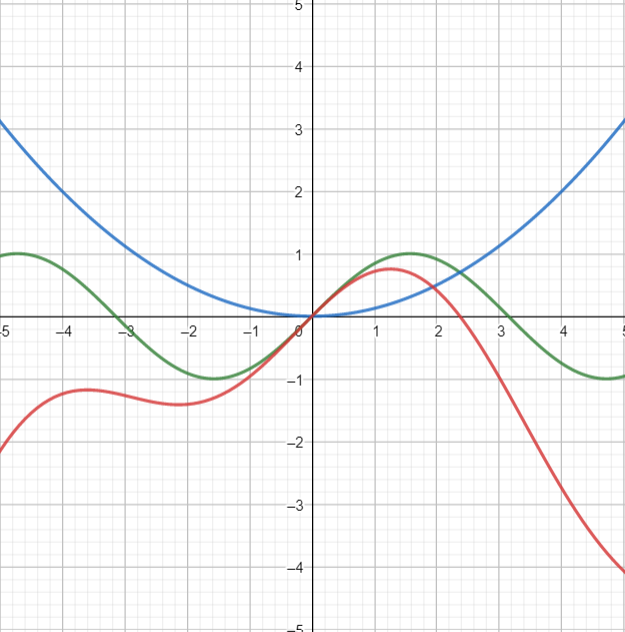
\includegraphics[width=7cm]{wykresy.png}
\end{minipage}
\hfill
\begin{minipage}[b]{3cm}
\centering
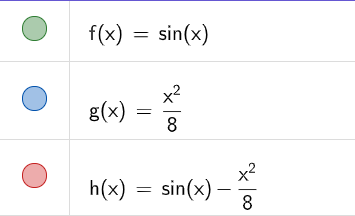
\includegraphics[width=4cm]{do_wykresow.png}
\end{minipage}
\caption{Wykres funkcji, stworzony przy użyciu geogebra.org/calculator}
\label{rys1}
\end{center}
\end{figure}

\section{Wyniki}
\textbf{4.1 Metoda siecznych}
\newline\newline
a) Dane zebrane podczas 15 iteracji dla $x_0=-8$ i $x_0=-8.1$ :

\begin{table}[h!]
    \centering
    \begin{tabular}{|c|c||c||c|} \hline
     & x & f(x) & f'(x) \\ \hline
1 & -3.05486 & -1.25315 & -9.17114\\ \hline
2 & -2.25638 & -1.41046 & -1.25315\\ \hline
3 & -9.41557 & -11.0908 & -1.41046\\ \hline
4 & -1.21327 & -1.12077 & -11.0908\\ \hline
5 & -0.291223 & -0.297725 & -1.12077\\ \hline
6 & 0.0423159 & 0.0420794 & -0.297725\\ \hline
7 & 0.00101238 & 0.00101225 & 0.0420794\\ \hline
8 & -5.6969e-06 & -5.69691e-06 & 0.00101225\\ \hline
9 & 7.21988e-10 & 7.21988e-10 & -5.69691e-06\\ \hline
10 & 5.14133e-16 & 5.14133e-16 & 7.21988e-10\\ \hline
11 & -4.63998e-26 & -4.63998e-26 & 5.14133e-16\\ \hline
12 & 0 & 0 & -4.63998e-26\\ \hline
13 & 0 & 0 & 0\\ \hline
14 & -nan & -nan & 0\\ \hline
15 & -nan & -nan & -nan\\ \hline
    \end{tabular}

    \label{tab:my_label}
\end{table}

\begin{figure}[h!]
\centering
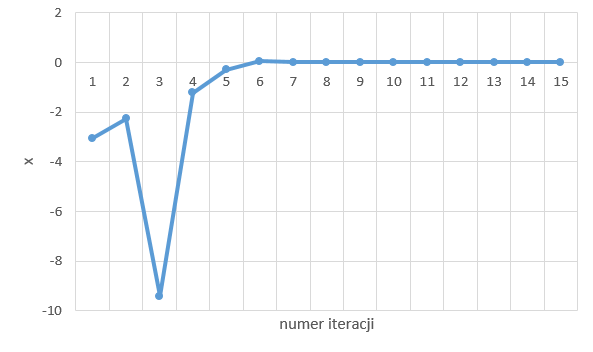
\includegraphics[width=9cm]{su.png}
\caption{ Wykres funkcji przybliżenia miejsca zerowego}
\label{fig:obrazek su}
\end{figure}
\newpage

b) Dane zebrane podczas 15 iteracji dla $x_0=8$ i $x_0=8.1$ :

\begin{table}[H]
    \centering
    \begin{tabular}{|c|c||c||c|} \hline
     & x & f(x) & f'(x) \\ \hline
1 & 4.82372 & -3.90234 & -7.23136\\ \hline
2 & 0.983196 & 0.711439 & -3.90234\\ \hline
3 & 1.5754 & 0.689754 & 0.711439\\ \hline
4 & 20.4119 & -51.0807 & 0.689754\\ \hline
5 & 1.82636 & 0.550569 & -51.0807\\ \hline
6 & 2.02455 & 0.386457 & 0.550569\\ \hline
7 & 2.49125 & -0.170328 & 0.386457\\ \hline
8 & 2.34848 & 0.0231226 & -0.170328\\ \hline
9 & 2.36554 & 0.000990854 & 0.0231226\\ \hline
10 & 2.36631 & -6.49953e-06 & 0.000990854\\ \hline
11 & 2.3663 & 1.79524e-09 & -6.49953e-06\\ \hline
12 & 2.3663 & 3.33067e-15 & 1.79524e-09\\ \hline
13 & 2.3663 & -1.11022e-16 & 3.33067e-15\\ \hline
14 & 2.3663 & -1.11022e-16 & -1.11022e-16\\ \hline
15 & -nan & -nan & -1.11022e-16\\ \hline

    \end{tabular}

    \label{tab:my_label}
\end{table}

\begin{figure}[H]
\centering
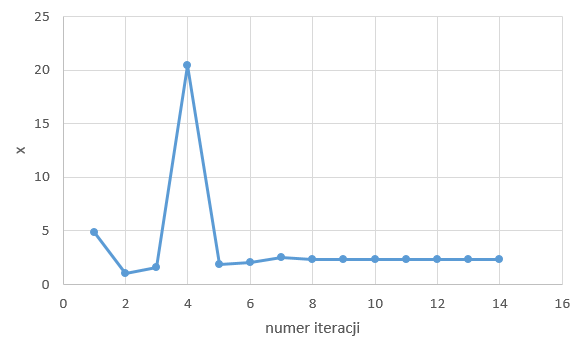
\includegraphics[width=9cm]{sd.png}
\caption{ Wykres funkcji przybliżenia miejsca zerowego}
\label{fig:obrazek sd}
\end{figure}

\newpage
\textbf{4.2 Metoda Newtona}
\newline\newline
a) Dane zebrane podczas 10 iteracji dla $x=-8$ :

\begin{table}[H]
    \centering
    \begin{tabular}{|c|c||c||c|} \hline
     & x & f(x) & f'(x) \\ \hline
1 &-3.15268 &  -1.23134 & -0.211769\\ \hline
2 & -8.96721  & -10.4931  &  1.34467\\ \hline
3 & -1.16374 &  -1.08757 &  0.686846\\ \hline
4 & 0.419697 &  0.385465 &  0.808288\\ \hline
5 & -0.0571942 & -0.0575719  &  1.01266\\ \hline
6 & -0.000342219 & -0.000342234 &   1.00009\\ \hline
7 & -1.46247e-08 & -1.46247e-08 &         1\\ \hline
8 & -2.67351e-17 & -2.67351e-17  &        1\\ \hline
9 & 0      &    0       &   1\\ \hline
10 & 0    &      0       &   1\\ \hline
    \end{tabular}

    \label{tab:my_label}
\end{table}

\begin{figure}[H]
\centering
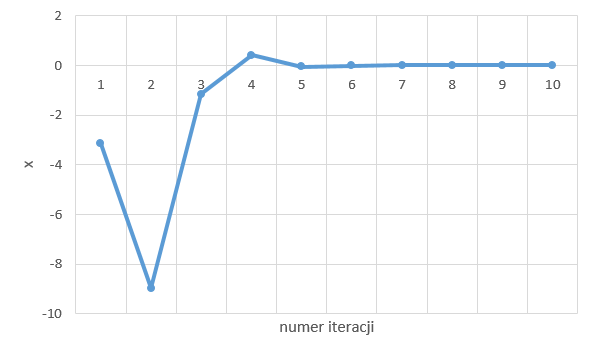
\includegraphics[width=9cm]{Nu.png}
\caption{ Wykres funkcji przybliżenia miejsca zerowego}
\label{fig:obrazek Nu}
\end{figure}
\newpage
b) Dane zebrane podczas 10 iteracji dla $x_0=8$ :

\begin{table}[H]
    \centering
    \begin{tabular}{|c|c||c||c|} \hline
     & x & f(x) & f'(x) \\ \hline
    1 & 4.7324 &  -3.79925 &  -1.16309\\ \hline
2 & 1.46589 &  0.725898  & -0.26176\\ \hline
3 & 4.23903 &  -3.13621 &  -1.51564\\ \hline
4 & 2.16979 &  0.237404  & -1.10626\\ \hline
5 & 2.38439 & -0.023775  & -1.32286\\ \hline
6 & 2.36642 & -0.000152012  &  -1.3059\\ \hline
7 & 2.3663 & -6.43529e-09 &  -1.30579\\ \hline
8 & 2.3663 & -1.11022e-16  & -1.30579\\ \hline
9 & 2.3663 & -1.11022e-16  & -1.30579\\ \hline
10 & 2.3663 & -1.11022e-16  & -1.30579\\ \hline
    \end{tabular}

    \label{tab:my_label }
\end{table}

\begin{figure}[H]
\centering
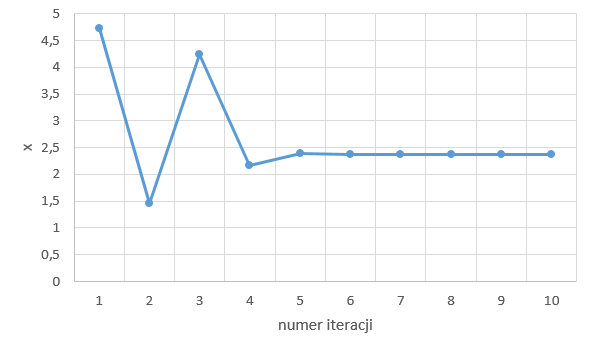
\includegraphics[width=9cm]{Nd.png}
\caption{ Wykres funkcji przybliżenia miejsca zerowego}
\label{fig:obrazek Nd}
\end{figure}

\newpage
\section{Wnioski}
\begin{flushleft}

By nie wykonywać zbędnych iteracji można wprowadzić warunek STOP-u polegający na przerwaniu pętli jeżeli
poprzednie przybliżenie rozwiązania nie różni się od aktualnego o więcej niż pewne bardzo małe $\epsilon$, spełnioy zostanie warunek: $|x_k_+_1-x_k| < \epsilon$.
\newline\newline
Kolejne przybliżenia zdają się w początkowych iteracjach oscylować wokół wartości teoretycznej. Wynika to z tego, że wyraz odejmowany od poprzedniego przybliżenia metodzie siecznych orazw metodzie Newtona, jest czasami naprzemiennie dodatni lub ujemny w kolejnych iteracjach algorytmu.
\newline\newline
Jak widać powyżej metoda Newtona daje nam lepsze rezultaty niż metoda siecznych. Dochodzi do szybszej stabilizacji wyników oraz finalnie dokładniejszego wyniku otrzymanego. Może to być spowodowane, że dzieleniem przez zero we wzorze na kolejne przybliżenie rozwiązania
\newline\newline
Metoda Newtona okazała się być szybsza od metody siecznych, gdyż udało się uzyskać bardzo dobre przybliżenie rozwiązania w mniejszej liczbie iteracji.

\end{flushleft}

\end{document}
